
\title{T-61.5130 Machine Learning and Neural Networks}
\author{Karhunen, Luttinen}
\date{Exercise 1, 2.11.2012}

\newcommand{\vect}[1]{{\bf{#1}}}
\newcommand{\svect}[1]{\boldsymbol{#1}}
\newcommand{\matr}[1]{\boldsymbol{#1}}

\usepackage{cancel}

\begin{document}

\maketitle

\begin{enumerate}

\item

  An odd sigmoid function is defined by
  \begin{equation}
    \label{eq:sigmoid}
    \varphi(v)=\frac{1-e^{-av}}{1+e^{-av}}=\tanh(av/2),
  \end{equation}
  where $\tanh$ denotes a hyperbolic tangent. The limiting values of
  this second sigmoid function are $-1$ and $+1$. Show that the
  derivative of $\varphi(v)$ with respect to $v$ is given by
  \begin{equation*}
    \frac{d\varphi}{dv}=\frac{a}{2}(1-\varphi^2(v)).
  \end{equation*}
  What is the value of this derivate at the origin? Suppose that the
  slope parameter $a$ is made infinitely large. What is the resulting
  form of $\varphi(v)$?  
  
  \begin{solution}

    The derivative of $\varphi(v)$:
    \begin{align*}
      \frac{d\varphi}{dv} &= \frac{a e^{-av} (1 + e^{-av}) + a
        e^{-av} (1 - e^{-av})} {(1+e^{-av})^2}
      && \text{Derivate using quotient rule}
      \\
      &= a \cdot \frac{ e^{-av} + \cancel{e^{-2av}} + e^{-av} -
        \cancel{e^{-2av}}} {(1 + e^{-av})^2}
      && \text{Cancel terms}
      \\
      &= \frac{a}{2} \cdot \frac{4 e^{-av}} {(1+e^{-av})^2} &&
      \text{Multiply numerator by 2}
      \\
      &= \frac{a}{2} \cdot \frac{1+2e^{-av}+e^{-2av} -
        1+2e^{-av}-e^{-2av}} {(1+e^{-av})^2} && \text{Add extra
        terms that sum to zero}
      \\
      &= \frac{a}{2} \cdot \frac{(1+e^{-av})^2 - (1-e^{-av})^2}
      {(1+e^{-av})^2} && \text{Re-organize terms}
      \\
      &= \frac{a}{2} \left[ 1 - \frac{(1-e^{-av})^2} {(1+e^{-av})^2}
      \right]
      \\
      &= \frac{a}{2} ( 1 - \varphi^2(v) )
    \end{align*}

    At the origin: 
    \begin{equation*}
      \left.\frac{d\varphi}{dv}\right|_{v=0} = \frac{a}{2} \left[1 - \left(
          \frac{1 - e^{-a * 0}}{1 + e^{-a*0}} \right)^2\right] = \frac{a}{2}.
    \end{equation*}
    \begin{equation*}
      \text{When  $a$ $\rightarrow$ $\infty$,  $\varphi(v)$ $\rightarrow$}
        \begin{cases}
          +1, &v > 0 \\
          -1, &v < 0 \\
          0, &v = 0
        \end{cases}
    \end{equation*}

    Fig.~\ref{fig:sigmoid} shows the values of the sigmoid function
    $\varphi(v)$ with different values of $a$.

    \begin{figure}[h]
      \begin{center}
        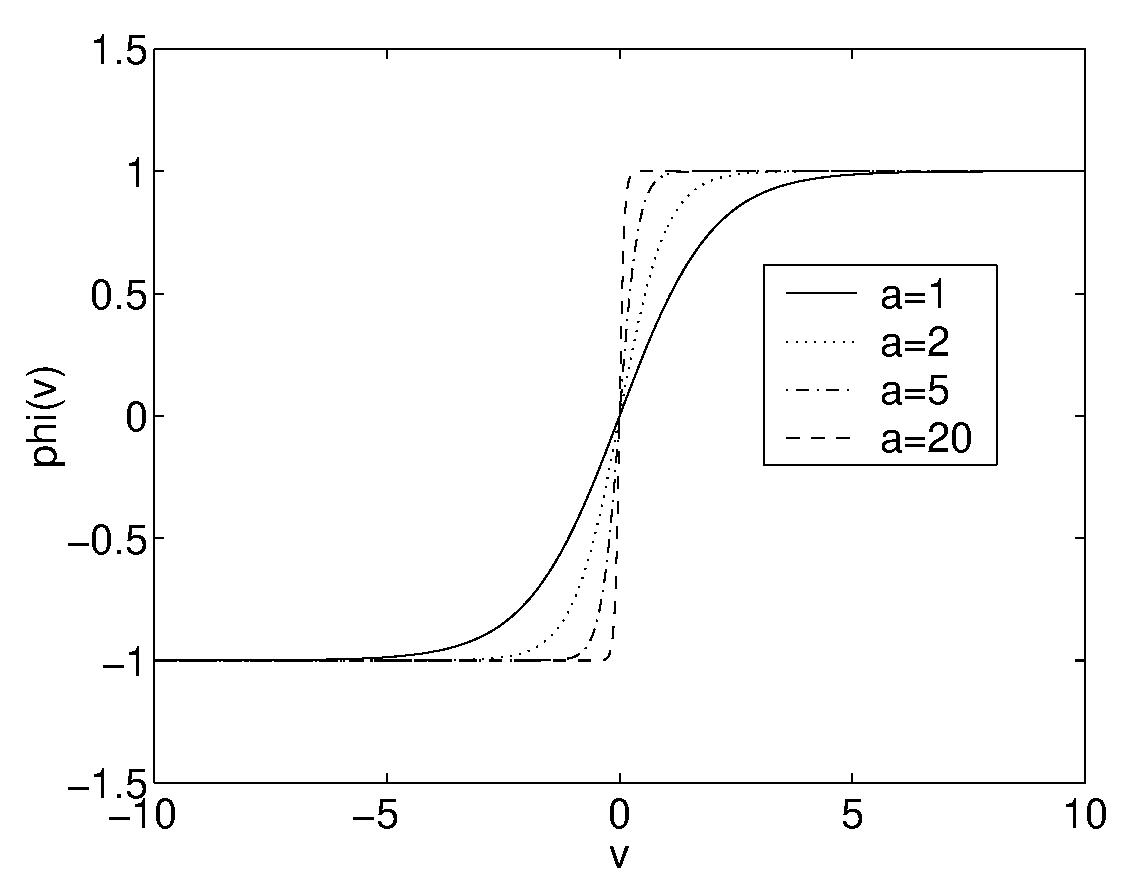
\includegraphics[width=12cm]{sigmoid.eps}
        \caption{\label{fig:sigmoid} Sigmoid function $\varphi(v)$ with
          different values of $a$. The function behaves linearly near the
          origin.}
      \end{center}
    \end{figure}

  \end{solution}
  
  
\item

  \begin{enumerate}
  \item Show that the McCulloch-Pitts formal model
    of a neuron may be approximated by a sigmoidal neuron (i.e.,
    neuron using a sigmoid activation function with large synaptic
    weights).
  \item Show that a linear neuron may be approximated by a sigmoidal
    neuron with small synaptic weights.
  \end{enumerate}
  
  \begin{solution}

    \begin{enumerate}
      
    \item The McCulloch-Pitts formula of a neuron is
      defined as a threshold function:
      \begin{equation}
        \varphi(v) = \left\{ \begin{array}{rl} 1, & v \geq 0 \\ 0, & v <
            0 \end{array} \right.,
      \end{equation}
      where $v_k = \sum_{j=1}^{m} w_{kj} x_j + b_k$, where $w_{kj}$'s are
      the synaptic weights and $b_k$ is the bias.
      
      A sigmoid activation function on interval $[0,1]$ is {\em e.g.}
      $\sigma(v) = 1 / (1 + e^{-av})$, where we assume $a > 0$ without
      loss of generality.
      
      When synaptic weights have large values, also $|a v|$ tends to have
      a large value:
      \begin{equation}
        \begin{aligned}
          \lim_{a \rightarrow \infty} \sigma(v)& = \left. \frac{1}{1 +
              e^{-av}}\right|_{a \rightarrow \infty} = \frac{1}{1+0} = 1 \mbox{\ \ \ \ \ \ ($v>0$)}
          \\
          \lim_{a \rightarrow \infty} \sigma(v)& = \left. \frac{1}{1 +
              e^{-av}}\right|_{a \rightarrow \infty} =
          \frac{1}{1-\infty} = 0 \mbox{\ \ \ \ \ ($v<0$)}
        \end{aligned}
      \end{equation}
      
    \item We expand the $e^{-av}$ in Taylor series around point $v=0$:
      
      \begin{equation}
        \begin{split}
          \sigma(v) &= \frac{1}{1 + e^{-av}} = \frac{1}{1 + 1 - av +
            \underbrace{\frac{(av)^2}{2!} - \frac{(av)^3}{3!} +
              \cdots}_{\mbox{$\approx$ $0$, for small values of $v$}}} \\ 
          &\approx \frac{1}{2 ( 1 - \frac{av}{2})} \\
          &= \frac{1}{2} \frac{1 + \frac{av}{2}} {1 -
            \underbrace{\frac{(av)^2}{4}}_{\approx 0}} \approx \frac{1}{2}
          \left(1 + \frac{av}{2} \right) = L(v) \: _\Box
        \end{split}
      \end{equation}
      
    \end{enumerate}

  \end{solution}
  

\item

  Consider a multilayer feedforward network, all the neurons of which
  operate in their linear regions. Justify the statement that such a
  network is equivalent to a single-layer feedforward network.

  \begin{solution}
    A single neuron is depicted in Fig.~\ref{fig:singleneuron}


    \begin{figure}[hb]
      \begin{center}
        % use '../process_fig.sh neuron.fig' to make the .pstex_t
        \input neuron.pstex_t
        \caption{\label{fig:singleneuron} A single sigmoidal neuron.}
      \end{center}
    \end{figure}
    
    There the input $v_k$ to the nonlinearity $\varphi$ is defined as
    $v_k = \sum_{j = 0}^n w_{kj}x_j = \vect{w}_k^T \vect{x}$, \newline
    where $\vect{x}=\begin{pmatrix} 1 & x_1 &\cdots & x_n
    \end{pmatrix}^T$ and $\vect{w}_k=\begin{pmatrix} w_{k0} &\cdots &
      w_{kn} \end{pmatrix}^T$.

    When the neuron operates in its linear region, $\varphi(v) \approx
    \alpha v$ and $y_k \approx \alpha \vect{w}_k^T \vect{x}$. For the
    whole layer, this gives: 

    \begin{equation}
      \vect{y} = \begin{pmatrix}  y_1 \\ \cdots \\ y_m \end{pmatrix}
      \approx \alpha \begin{pmatrix}  \vect{w}_1^T \vect{x}\\ \cdots \\
        \vect{w}_m^T \vect{x} \end{pmatrix} 
      = \alpha \begin{pmatrix}  \vect{w}_1^T\\ \cdots \\
        \vect{w}_m^T \end{pmatrix} \vect{x} = \matr{W} \vect{x},
    \end{equation}
    where
    \begin{equation}
      \matr{W} = \alpha \begin{pmatrix}
        w_{10} & \cdots & w_{1n} \\ \vdots & \ddots & \vdots \\
        w_{m0} & \cdots & w_{mn} 
      \end{pmatrix}
    \end{equation}
    
    The whole network is constructed from these single layers:

    \begin{center}
      % use '../process_fig.sh network.fig' to make the .pstex_t
      \input network.pstex_t
    \end{center}
    
    and the output of the whole network is

    \begin{equation}
      \vect{y} = \matr{W_N} \vect{u_{N-1}} = \matr{W_N}  \matr{W_{N-1}}
      \vect{u_{N-2}} = \prod_{i = 1}^{N} \matr{W_i} \vect{x}.
    \end{equation}

    The product $\matr{T} = \prod_{i = 1}^{N} \matr{W_i}$ is a matrix of
    size $m \times n$: 

    \begin{equation}
      \vect{y} = \matr{T} \vect{x} = 
      \begin{pmatrix}
        t_{10} & \cdots & t_{1n} \\ \vdots & \ddots & \vdots \\
        t_{m0} & \cdots & t_{mn} 
      \end{pmatrix} \vect{x} = 
      \begin{pmatrix}  \vect{t}_1^T\\ \cdots \\
        \vect{t}_m^T 
      \end{pmatrix} \vect{x},
    \end{equation}
    
    which is exactly the output of a single layer linear network having
    $\matr{T}$ as the weights $_\Box$

  \end{solution}
  
\item

  \begin{enumerate}
  \item Construct a recurrent neural network which has two neurons in
    the input layer plus bias terms, and 3 neurons in the hidden layer
    having recurrent connections with self-feedback.  The output of
    the network is the output of the first hidden neuron.
  \item Write the equations describing the operation of this network.
  \end{enumerate}

  \begin{solution}
    \begin{enumerate}
    \item \      
      \begin{center}
        \usetikzlibrary{shapes}
        \usetikzlibrary{chains}
        \usetikzlibrary{arrows}
        \begin{tikzpicture}[start chain=hidden going below,
          start chain=input going below]

          \tikzset{>={triangle 45}}
          
          % 
          \foreach \i in {1,...,6} {
            \node[rectangle,draw] (in\i) at (0,2*7-2*\i) {};
          }
          \foreach \i in {1,...,3} {
            \node[circle,draw,fill=gray,minimum size=20pt] (hid\i) at (3,2*5.5-2*\i) {};
          }
          % 
          % % Hidden layer
          % \node[circle,fill=gray!25,draw,minimum
          % size=20pt,on chain=hidden,label=1] (h1) {};
          % \node[circle,fill=gray!25,draw,minimum
          % size=20pt,on chain=hidden,label=2] (h2) {};
          % \node[circle,fill=gray!25,draw,minimum
          % size=20pt,on chain=hidden,label=3] (h3) {};
          % 

          % Output layer
          \node[right=100pt of hid1]
          (out) {$y(n)$};

          % Arrows input->hidden
          \foreach \i in {1,...,6} {
            \foreach \j in {1,...,3} {
              \draw[->] (in\i) -- (hid\j);
            }
          }

          % Arrow hidden->output
          \draw[->] (hid1) -- (out);

          % Recurrent arrows
          \foreach \i in {1,2,3} {
            % Unit time-delays
            \path (hid\i) ++(-1.5,3*\i+2) node[draw,rectangle,minimum
            size=20pt] (z\i) {$z^{-1}$};
            % Arrows
            \draw[->] (hid\i) -- ++(1.5+\i*0.5,0) node[at start,label=above
            right:$x_\i(n)$] {} node (crossing\i) {} -- ++(0,3*\i+2) --
            (z\i) -- ++(-\i*0.5-3,0) node (current) {} -- (current |- in\i)
            -- (in\i) node[at end, label=above left:$x_\i(n-1)$] {};
          }

          \node[circle,draw,fill,scale=0.4] at (crossing1) {};

          \draw[<-] (in4) -- ++(-1,0) node[label=left:$1$] {};
          \draw[<-] (in5) -- ++(-1,0) node[label=left:$u_1(n)$] {};
          \draw[<-] (in6) -- ++(-1,0) node[label=left:$u_2(n)$] {};
          
        \end{tikzpicture}
      \end{center}

    \item
        
      There are two neurons in the input layer, three neurons in the
      hidden layer and one output. In the following, we consider a
      more general case with arbitrary number of neurons in each
      layer.

      Let the $q$-by-$1$ vector
      $\mathbf{x}(n)=[x_1(n),\,\ldots,\,x_q(n)]^{\mathrm{T}}$ denote
      the state vector of recurrent network. Let the $(m+1)$-by-$1$
      vector $\mathbf{u}(n)$ denote the input applied to the system
      and the constant $1$ is concatenated into this vector
      $\mathbf{u}(n)=[1,\,u_1(n),\,u_2(n),\,\ldots,\,u_m(n)]^{\mathrm{T}}$.
      The $p$-by-$1$ vector $\mathbf{y}(n)$ denotes the corresponding
      output of the system.  In mathematical terms, the dynamic
      behavior of the system, assumed to be noise free, is described
      by the following pair of nonlinear equations:
      \begin{align*}
        \mathbf{x}(n) &= \boldsymbol\phi \left( \mathbf{W}_a \mathbf{x}(n-1) +
          \mathbf{W}_b \mathbf{u}(n) \right), \\
        \mathbf{y}(n) &= \mathbf{C} \mathbf{x}(n),
      \end{align*}
      where $\mathbf{W}_a$ is a $q$-by-$q$ matrix, $\mathbf{W}_b$ is a
      $q$-by-($m+1$) matrix, $\mathbf{C}$ is a $p$-by-$q$ matrix and
      $\boldsymbol\phi: \mathbb{R}^q \rightarrow \mathbb{R}^q$ is a diagonal map
      described by

      \[
      \boldsymbol{\phi}:
      \left[\begin{array}{c}
          x_1 \\
          x_2 \\
          \vdots \\
          x_q
        \end{array}\right]
      \rightarrow
      \left[\begin{array}{c}
          \phi(x_1) \\
          \phi(x_2) \\
          \vdots \\
          \phi(x_q)
        \end{array}\right]
      \]
      for some memoryless, component-wise nonlinearity $\phi$.
      % : \mathbb{R}^m$,
      % $\mathbb{R}^n$, and $\mathbb{R}^p$ are called the input space, state
      % space, and output space, respectively.

      In the network of the figure we have $m$=2, $q$=3 and $p$=1. Thus the
      matrices $\mathbf{W}$ are defined as follows

      \[
      \mathbf{W}_a = 
      \left[\begin{array}{ccc}
          w_{11} & w_{12} & w_{13} \\
          w_{21} & w_{22} & w_{23} \\
          w_{31} & w_{32} & w_{33} \\
        \end{array}\right]
      \]

      \[
      \mathbf{W}_b = 
      \left[\begin{array}{ccc}
          b_{1} & w_{14} & w_{15} \\
          b_{2} & w_{24} & w_{25} \\
          b_{3} & w_{34} & w_{35} \\
        \end{array}\right]
      \]

      where the first column of $\mathbf{W}_b$ represents the bias terms applied to
      neurons 1, 2 and 3. The matrix $\mathbf{C}$ is defined by

      \[
      \mathbf{C} = [1, \; 0, \; 0]
      \]
    \end{enumerate}
  \end{solution}
  
\end{enumerate}





\end{document}             % End of document.
